\chapter{Digital signature schemes}
\label{chpr:dss}

In this chapter we will present the general idea behind digital signatures: what they are and why they are used. Then we will discuss the Elliptic Curve Digital Signature Algorithm (ECDSA), the one actually used in Bitcoin. After having delved into its problems, we will present the adaptation of the Schnorr signature to elliptic curve cryptography (there is currently a discussion about its adoption in Bitcoin). The comparison will turn out to be pitiless.
\\
For a detailed explanation of how signatures are actually used in Bitcoin we refer to Appendix \ref{app:A}.
\\
\\
To understand what a digital signature scheme is, we start considering the situation in which Alice wants to sign a document that she aims sending to Bob, who wants assurance that the document comes from Alice and has not been tampered with. As for real life signatures, the aim of a proper digital signature scheme should be to prove the authenticity of a message or document, in the digital realm. Thus, we can list some properties that a proper scheme should provide:
\begin{itemize}
	\item Authentication: gives a recipient reasons to believe that the message was created by a known sender;
	\item Non repudiation: the sender cannot deny having sent the message;
	\item Integrity: ensures that the message has not been altered.
\end{itemize}
A naive approach to this problem would be to digitalize Alice's signature: but in this case it would be too easy for an eavesdropper to simply copy her signature and append it to another document. 
\\
In order to achieve the listed properties, as first thing we should tie the signature to the document, so that it could not be used again: this would also solve the problem of integrity. If the message changes, the signature is not valid anymore.  Moreover, it should be possible for someone to verify that the signature is valid, and it should be possible to show that Alice must have been the person who signed the document: this would ensure the authentication and non repudiation properties. 
\\
In cryptography usually some security models are introduced for the so called unforgeability, the property that prevents adversaries from being able to forge a signature that seems to come from Alice. In particular we consider the security model known as existentially unforgeability under chosen message attack, where forgery means winning at the following game:
\begin{enumerate}
	\item The signer (Alice) gives her public key to the adversary (also known as forger or attacker);
	\item The adversary sends messages $m_i$ to the challenger (Alice) and receives valid signature $\sigma$ on the message $m_i$ for the given public key. He may do this as many times as he likes;
	\item The adversary produces a message $m \neq m_i, \ \forall i$ (i.e. the message has not been queried before) along with a valid signature on it.
\end{enumerate}
In this model, unforgeability means that no computationally bounded adversary is able to forge a signature except with negligible probability: in this setting a forgery consists in a signature for a message/public key pair never queried. This hypothesis can be relaxed, excluding from the winning conditions only the triplets message/public key/signature obtained from a query, leading to the concept of strong unforgeability under chosen message attack (SUF-CMA).

\bigskip
\noindent
Now that we have presented the security model, we can look more formally at the scheme: a signature scheme is a triplet of algorithms $(KeyGen, Sign, Ver)$, where the first two are randomized algorithms, while the third one is deterministic. To sign a document or message, the signers proceeds as follows:
\begin{itemize}
	\item He runs the key generation algorithm with no inputs\footnote{Some authors consider as input a security parameter, but we take it as given.} to generate a key pair: $(q, Q) = KeyGen()$;
	\item He runs the signing algorithm on message $m$ and private key $q$, resulting in a signature $\sigma$: $\sigma = Sign(m, q)$;
	\item A verifier can easily check the validity of the signature running the verification algorithm as follows: $Ver(\sigma, m, Q) \in \{0, 1\}$. If $Ver(\sigma, m, Q) = 1$ then the signature is valid, otherwise it is not.
\end{itemize}
A proper signature scheme should satisfy the following consistency equation: $Ver(Sign(m,q), m, Q) = 1, \ \forall (q, Q)$ returned from the key generation algorithm.
\\
A possibility to construct a signature scheme relies on the difficulty of discrete logarithms on elliptic curves. In the next sections we will analyse deeply merits and flaws of two schemes constructed on this hypothesis.

\bigskip

\section{Elliptic curve digital signature algorithm (ECDSA)}
Assume that Alice wants to sign a message $M$ and send it to Bob. The first thing to do for the parties involved is to agree on an elliptic curve determined by the set of parameters $T$ and on a cryptographically secure hash function. This function is used to get a digest from $M$: indeed, a digital signature can only sign small amounts of data. Applying a proper hash function to a message produces a digest which is small enough and that can act as digital fingerprint if the output space is large enough. Now Alice chooses a secret integer $q_A \in [1, ..., n - 1]$ (the private key) and computes her public key $Q_A = q_AG$, that sends to Bob who has to validate it (Alice shouldn't be able to repudiate the signature due to the use of an invalid public key). 
\\
The public key can be made public thanks to the difficulty of the ECDLP; moreover, the fact that it is public allows anyone to verify Alice's signature, constituting the non repudiation property.
\\
Now that we have talked about the setup procedure we can give a closer look to the signing and verification algorithms.

\bigskip

\begin{algorithm}
	\caption{ECDSA: signing algorithm}
	\label{alg:ecdsa_sig}
	\begin{algorithmic}[1]
		\Procedure{ecdsa\_sig}{$M, \ q$}
		\State $m \gets \text{hash}(M)$
		\State Let $z$ be the $L_n$ leftmost bits of $m$: $z \gets \text{int}(z)$
		\State $k \xleftarrow{\text{\$}} [1, ..., n - 1]$
		\State $K = kG = (x_K, y_K)$
		\State $r = x_K \ (\text{mod} \ n)$
		\If {$r = 0$}
		\State \textbf{go to} step 4
		\EndIf 
		\State $s = k^{-1}(z + rq_A) \ (\text{mod} \ n)$
		\If {$s = 0$}
		\State \textbf{go to} step 4
		\EndIf
		\State \textbf{return} $(\text{bytes}(r), \text{bytes}(s))$
		\EndProcedure
	\end{algorithmic}
\end{algorithm}

\bigskip

\begin{algorithm}
	\caption{ECDSA: verification algorithm}
	\label{alg:ecdsa_ver}
	\begin{algorithmic}[1]
		\Procedure{ecdsa\_ver}{$(r, s), M, Q\ $}
		\State $r \gets \text{int}(r)$, $s \gets \text{int}(s)$
		\If {$r \notin [1, ..., n - 1]$ or $s \notin [1, ..., n - 1]$}
		\State \textbf{return} {\bf False}
		\EndIf
		\State $m \gets \text{hash}(M)$
		\State Let $z$ be the $L_n$ leftmost bits of $m$: $z \gets \text{int}(z)$
		\State $u_1 \gets zs^{-1} \ (\text{mod} \ n)$, $u_2 \gets zrs^{-1} \ (\text{mod} \ n)$
		\State $K \gets u_1G + u_2Q_A$
		\If {$K = \infty$}
		\State \textbf{return False} 
		\EndIf
		\State \textbf{return $r = x_K \ (\text{mod} \ n)$}
		\EndProcedure	
	\end{algorithmic}
\end{algorithm}

\bigskip
\noindent
It is necessary for $k$ not only to be secret, but to be selected differently each time: otherwise the secret key would be recoverable. Indeed, let's consider two signatures on different messages $(r, s)$ and $(r, s')$ derived using the same $k$. After having converted $r, s$ and $s'$ to integers, we have:
$$s = k^{-1}(z + rq_A) \ (\text{mod} \ n), \ s' = k^{-1}(z' + rq_A) \ (\text{mod} \ n) \ \Longrightarrow $$ $$\Longrightarrow s - s' = k^{-1}(z - z') \ (\text{mod} \ n) \ \Longrightarrow \ k = (z - z')(s - s')^{-1} \ (\text{mod} \ n).$$
From just two signatures we were able to recover the common $k$ and now we can derive the private key from the definition of $s$ or from the definition of $s'$:
$$q_A = r^{-1}(ks - z) \ (\text{mod} \ n).$$
\\
To ensure that $k$ is unique for each message one may bypass random number generation completely, since it is one of the main sources of problems in cryptosystems, and generate deterministic signatures by deriving $k$ from both the message and the private key as: $k = \text{hash}(q \ || \ m)$.
\\
Moreover there are some ways to speed up the verification procedure: through the Shamir’s trick, the sum of two scalar multiplication can be calculated faster than the two isolated scalar multiplication at point nine. Finally, we can speed up the verification procedure further, by making $K$ efficiently recoverable from $r$. In this case one may verify that $sR = zG + rQ_A$. This can be done by including the point $R$ itself in the signature, either in compressed ($x_R$ coordinate and a byte telling the sign of $y_R$, $0\text{x}02$ or $0\text{x}03$ if is is even or odd, respectively) or uncompressed form.

\bigskip
\noindent
Let's give a look now at the proof of the verification algorithm correctness.
\\
{\bf Proof of correctness}: We have to prove that $kG = K = u_1G + u_2Q_A$.
\begin{itemize}
	\item From the definition of $Q_A$: $u_1G + u_2Q_A = u_1G + u_2q_AG$;
	\item From the definition of $u_1$ and $u_2$: $u_1G + u_2Q_A = s^{-1}(z + rq_A)G$;
	\item From the definition of $s$: $u_1G + u_2Q_A = (k^{-1}(z + rq_A))^{-1}(z + rq_A)G = k(z + rq_A)^{-1}(z + rq_A)G = kG$.
\end{itemize}
\ \ \ \ \ \ \ \ \ \ \ \ \ \ \ \ \ \ \ \ \ \ \ \ \ \ \ \ \ \ \ \ \ \ \ \ \ \ \ \ \ \ \ \ \ \ \ \ \ \ \ \ \ \ \ \ \ \ \ \ \ \ \ \ \ \ \ \ \ \ \ \ \ \ \ \ \ \ \ \ \ \ \ \ \ \ \ \ \ \ \ \ \ \ \ \ \ \ \ \ \ \ \ \ \ \ \ \ \ \ \ \ \ \ \ \ \ \ \ \ \ \ \ \ \ \ \ \ \ \ \ \ \ \ \ \ \ \ $\square$
At the beginning of the chapter we have said that the comparison between ECDSA and Schnorr will be pitiless, so it is clear that ECDSA is far from being perfect. Let's discuss some of its problems:
\begin{itemize}
	\item Malleability: the signature $(r, s)$ may be replaced with $(r, -s \ (\text{mod} \ n))$, because this is an equivalent signature. This means that a third party, without access to the private key can alter an existing valid signature for a given public key and message into another signature that is valid for the same key and message. However this is not regarded as a forgery on the scheme since the message is the original one, but this possibility prevented the deployment of layer two solutions for the Bitcoin scalability problem (e.g. Lightning network). However in Bitcoin this problem has been solved through the soft fork SegWit.
	\\
	Augmenting the verification equation with the check $s \leq (n - 1) / 2$ we can make ECDSA strongly unforgeable (which prevents the malleability problem);
	\item The signing operation needs the calculation of the modular inverse of $k$ and as we have seen it is a slow operation. Moreover this computation can be done only if $n$ is a prime number. Indeed we have a theorem stating that $x \in \mathbb{Z}_n$ is invertible if and only if the greatest common divisor of $x$ and $n$ is one\footnote{\url{https://www.coursera.org/learn/crypto/lecture/2YWK8/notation}, from minute 7.39.}. This obviously holds true for every $x \in \mathbb{Z}_n$ if and only if n is a prime number. However this is not at all a problem, but just a remark: $n$ has to be a huge prime number for the ECDLP to be hard;
	\item In order for ECDSA to be secure, it can be shown that we need a small cofactor $h$. This is due to the presence of attacks on the conversion function used in the sixth step of the signing operation, the one that entails taking the $x$ coordinate of $K$ and reducing it modulo $n$. It is told in \cite{RefWork:2} that this function has to be almost bijective for ECDSA to be secure, which means that an attacker cannot find an $r$ for which a random $K$ has non negligible probability of satisfying $r = x_K \ (\text{mod} \ n)$. Indeed we have that the integers $x_K = r + jn$ for $j \in \{0, 1, 2, ..., h\}$, if $h = 1$ or 2 as recommended in \cite{RefWork:3}, are linked usually to one valid candidate $x$ coordinate.
\end{itemize}

\bigskip

\subsection{ECDSA: multi-signature}
Multi-signature schemes allow a group of users to cooperate (interactively or not) to sign a single message or document, usually producing a joint signature that is more compact than a collection of distinct signatures from all users. Verification usually requires the message $m$ and the set of public keys of the signers.
\\
Before we analyse ECDSA multi-signature, let's see formally what these schemes are.

\bigskip
\noindent
A multi-signature algorithm is a triplet of algorithms $(KeyGen, Sign, Ver)$. To sign jointly a document or message $m$, each participant $i$ of the scheme should proceed as follows:
\begin{itemize}
	\item She generates a public key pair through the key generation algorithm: $\{q_i, Q_i\} = KeyGen()$;
	\item She sends her public key to all the other participants, so that every user can gather the same multiset $L$ of public keys: $L = \{Q_1, Q_2, ..., Q_n\}$;
	\item She runs the signing algorithm on message $m$, secret key $q_i$ and multiset of public key $L$: $\sigma = Sign(m, q_i, L)$;
	\item A verifier can check the validity of the signature through the verification algorithm: $Ver(\sigma, m, L) \in \{0, 1\}$. If it returns 1 then the signature is valid, otherwise it is not.
\end{itemize}
A proper multi-signature scheme should output to every signer the same signature $\sigma$ that satisfies the following consistency equation: 
$$Ver(Sign(m, q_i, L), m, L) = 1, \ \forall q_i \ \text{s.t.} \ q_iG = Q_i \in L.$$
It is easy, given a signature scheme, to extend it to the multi-user setting in a naive way: each signer signs the message with its own private key, the final signature being the concatenation of the partial signatures. This is the approach used today in Bitcoin with ECDSA: the problem is that the signature size increase linearly in the number of participants. Ideally, the size of the signature should be independent of the number of participants, leading to higher fees for the users and a bloat of the blockchain size that affects every participant in the network.
\\
ECDSA multi-signatures requires multiple public keys in order to validate multiple signatures, i.e. despite the name, multi-signature in Bitcoin is just a tuple of distinct users' signatures.
\\
In literature, the name multi-signature is associated to schemes that, given $n$ participants, require the collaboration of everybody to produce a valid signature. In Bitcoin this notion is extended to the so called threshold schemes: if before we talked about $n$-of-$n$ schemes, these can be though of as $m$-of-$n$, where at least $m <= n$ participants have to collaborate to sign.

\bigskip

\subsection{ECDSA: public key recovery}
Given an ECDSA signature $(r, s)$ and EC domain parameters $T$, it is generally possible to determine the public key $Q$ associated to the private key used to generate the signature. This is useful in bandwidth constrained environments, when transmission of public keys cannot be afforded. Potentially, several candidate public keys can be recovered from a signature (their number is linked to the cofactor). The algorithm is presented in Algorithm \ref{alg:key_recovery}.

\begin{algorithm}
	\caption{ECDSA: public key recovery}
	\label{alg:key_recovery}
	\begin{algorithmic}[1]
		\Procedure{ecdsa\_recovery}{$(r, s), M$}
		\State $keys \gets \{\}$
		\State $r \gets \text{int}(r), \ s \gets \text{int}(s)$
		\For {$j \gets 0, h - 1$}
		\State $x \gets r + jn$
		\State $K \gets \text{EC\_point}(x)$. 
		\If {$K = {\bf False}$ or $nK \neq \infty$}
		\State \textbf{go to} step 3
		\EndIf
		\State $m = \text{hash}(M)$
		\State Let $z$ be the $L_n$ leftmost bits of $m$: $z \gets \text{int}(z)$
		\For {$k \gets 1,2$}
		\State $Q \gets r^{-1}(sK - zG)$
		\State $keys \gets keys + Q$
		\State $K \gets -K$
		\EndFor
		\EndFor
		\State \textbf{return} $keys$
		\EndProcedure
	\end{algorithmic}
\end{algorithm}
\noindent
In the set $keys$ there is the correct key. Authenticity could be checked against a public key in some certificate or directory.
\\
Through public key recovery, the verification of a signature becomes implicit: you first recover $Q$ from $(r, s)$. Then, the signature is deemed valid once the public key $Q$ has been authenticated. This step is necessary since, in general, from every signature we can extract a public key.

\bigskip

\bigskip

\section{Schnorr signature algorithm}
In this section we finally pass to analyse the core of the present work, following closely the recent Bitcoin Improvement Proposal by Pieter Wuille \cite{RefWork:5} on the standardization of the Schnorr signature\footnote{The BIP proposes a standardization of Schnorr but does not deal with the possible implementation in Bitcoin.}.
\\
As stated in the BIP, ECDSA is standardized, while the Schnorr signature, due to the presence of a patent in past years, is not. But the first one has some downsides compared to the latter over the same curve:
\begin{itemize}
	\item Security proof: the security of Schnorr signature is proved in the random oracle model\footnote{In the random oracle model (ROM) hash functions are modelled as truly random functions whose outputs are uniformly random and can be computed by querying a public oracle.} assuming the ECDLP is hard. Such a proof does not exist for ECDSA, since its security proof requires the generic group model. The two proofs can be found in \cite{RefWork:8} and \cite{RefWork:9}, respectively. The provably secure construction offered by Schnorr is important since it could prevent attacks from ECDSA in the future\footnote{This is a major achievement since Schnorr provides better security based on the same hypothesis: we do not need to introduce stronger conditions to improve the security.};
	\item Non-malleability: ECDSA, as already showed, is malleable. On the other hand, Schnorr signatures are provably non-malleable\footnote{Segregated witness (SegWit) solves the known malleability problems of ECDSA, but we do not know if others exist. On the other hand, Schnorr is strongly unforgeable under chosen message attacks (SUF-CMA).};
	\item Linearity: Schnorr verification algorithm is linear in both the terms of the signature, so that multiple parties can collaborate to produce a signature that is valid for the sum of their public keys (native multi-signature construction, discussed later on with its flaws).
\end{itemize}
Thanks to these characteristic, the introduction of Schnorr in Bitcoin would result in privacy and efficiency improvements. Moreover, thanks to the version system introduced by SegWit, Schnorr can be deployed "easily" through a soft fork. Schnorr signature could moreover enable easier implementation of higher level protocols, such as general payment channels and atomic swaps, for which we refer to a later chapter.

\bigskip
\noindent
The fact that Schnorr is not standardized, allows us to make design choices in order to implement other features in addition to the native ones:
\begin{itemize}
	\item Batch validation: the specific formulation of ECDSA signature that is standardized cannot be validated more efficiently in batch compared to individually. Switching to Schnorr offers the opportunity to choose a formulation that allows batch validation. This can be an important feature in Bitcoin since when validating a block we need to verify multiple signatures; moreover, we are interested that all of them are valid: if the verification fails, we do not care about which signature caused the failure. We simply reject the whole block;
	\item Fixed size: the proposed Schnorr standardization is of fixed size, 64 bytes. This is in contrast with the 70-72 bytes long ECDSA (caused by the DER encoding). This would lead to a reduction of on-chain transactions' size.
\end{itemize}
Even if we decided to be compliant with the BIP, we remark the fact that when signing with Schnorr there are two possible shape for the signature. EC Schnorr signatures for the message $m$ and public key $Q$ involve a point $K$ and integers $e$ and $s$ which satisfy $e = \text{hash}(K \ || \ m)$ and $sG = K + eQ$. The two different verification equation depend on whether we decide to include $e$ or $K$ in the signature.
\begin{itemize}
	\item The signature is $(e, s)$ with $e = \text{hash}(sG - eQ \ || \ m)$. This choice avoids the difficulty of encoding an EC point in the signature;
	\item The signature is $(K, s)$ with $sG = K + \text{hash}(K \ || \ m)Q$. This formulation supports batch validation since there are no elliptic curve operations inside the hashes.
\end{itemize}
The choice falls on the second option, since it supports batch validation. Batch validation is important also because it would speed up considerably the syncing of new Bitcoin nodes that have to download the entire blockchain and validate every transaction.
\\
However, using the second validation rule directly comes with a downside: it is possible for a third party to convert a signature $(K, s)$ for key $Q$ into a signature $(K, s + a*\text{hash}(K \ || \ m))$ for key $Q + aG$ and the same message, for any integer $a$. Indeed, the signature $(K, s)$ is verified checking that $sG = K + \text{hash}(K \ || \ m)Q$, thus: $(s + a*\text{hash}(K \ || \ m))G = sG + a*\text{hash}(K \ || \ m)G = K + \text{hash}(K \ || \ m)Q + a*\text{hash}(K \ || \ m)G = K + \text{hash}(K \ || \ m)(Q + aG)$.
This is not a concern for the Bitcoin protocol itself, due to the difficulty of the ECDLP\footnote{An adversary could convert the signature to a public key of his choice only knowing the secret key of the signer: in this way he would be able to compute $Q_{adv} = (q + a)G$, choosing properly the integer $a$.}. However it may be better to avoid this problem, since in some cases, such as unhardened key derived using BIP32, if Bob knows Alice's master public key, he would be able to transform Alice's signature under a parent public key into another for any public key derived from the same master public key. For this reason, the BIP suggests to use key prefixed Schnorr, changing the equation to $sG = K + \text{hash}(K \ || \ Q \ || \ m)Q$. Because any change in the public key would produce unpredictable changes in the hash, Bob cannot use an existing signature to do anything but verify it. Notice that this choice prevents the possibility for public key derivation, a construction that is typically incompatible with batch validation\footnote{\url{https://bitcoin.stackexchange.com/questions/77234/schnorr-vs-ecdsa}.}.
\\
Let's give a deeper look at how this formulation can be exploited in case of unhardened derivation using BIP32. Without entering in the details, in BIP32 it is specified how to derive key pairs from a unique master key pair, easing incredibly the backup procedure: the major achievement is that the whole tree of key pairs is recoverable from a special number called seed, that can be safely stored in efficient ways. We label the parent key pair as $(q_P, Q_P)$ and the child key pair as $(q_C, Q_C)$. The scheme for unhardened derivation is represented in Figure \ref{fig:bip32} and works as follows: we use the hash function HMAC, that outputs in the space of 512 bits, fed with the parent public key, the parent chain code (for our purposes the only thing that matters is that it is derived as half of the output of the HMAC function, i.e. it is a 256 bit string) and the child index. The result is divided in two half, an offset and the child chaincode (that will be needed for further derivations). The offset is added to the parent private key (modulo the order of the curve) to obtain the child private key. Thus, denoting the offset as $f$, we have the following relation: $q_C = f + q_P \ (\text{mod} \ n) \ \Longrightarrow \ Q_C = fG + Q_P$.

\begin{center}
	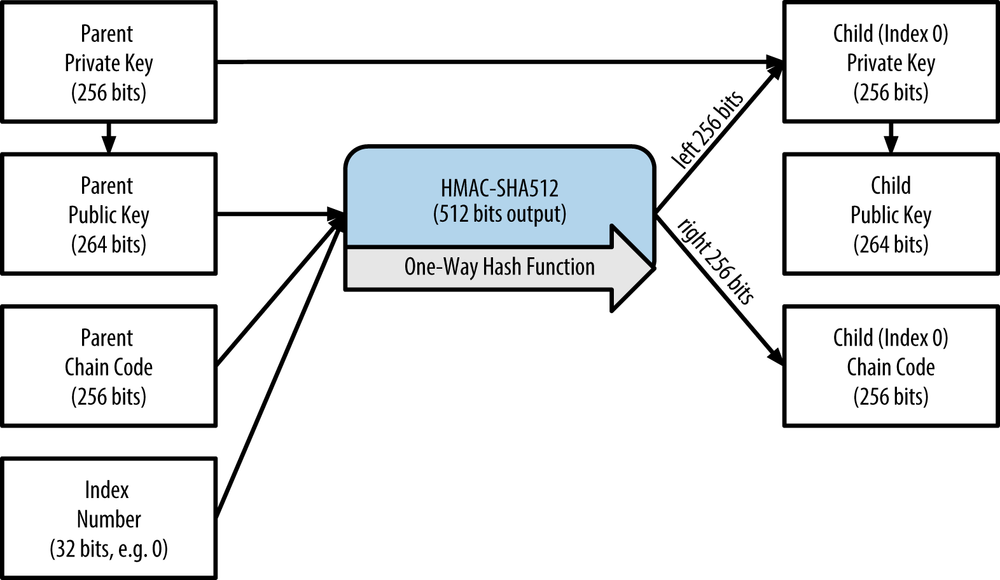
\includegraphics[scale = 0.4]{Images/bip32.png}
	\captionof{figure}{BIP32's unhardened derivation, source: \cite{RefWork:7}.}
	\label{fig:bip32}
\end{center}
Now, imagine an attacker is given a valid signature $(K, s)$ for public key $Q_P$ and message $m$. Relying on the previous relation, he is able to forge a valid signature for public key $Q_C$ and for the same message $m$ as $(K, s + \text{hash}(K \ || \ m)f)$. Indeed we have:
$$(s + \text{hash}(K \ || \ m)f)G = sG + \text{hash}(K \ || \ m)fG = $$
$$= K + \text{hash}(K \ || \ m)Q_P + \text{hash}(K \ || \ m)fG = K + \text{hash}(K \ || \ m)(Q_P + fG) = $$
$$ = K + \text{hash}(K \ || \ m)Q_C.$$
When substituting $sG$ with $K + \text{hash}(K \ || \ m)Q_P$ we relied on the fact that $(K, s)$ was a valid signature for public key $Q_P$ and message $m$. Notice that the attacker only needs a valid signature for the parent public key, the related public key and message, the parent chaincode and the child index.
\\
This is a particular case of the previously presented weakness, that now can be exploited since the relation between the two public keys is known. The hardened derivation also would prevent the forgery since, in place of the parent public key, the parent secret key is given as input to the hash function. To learn the relation between the two public keys, i.e. the offset, the forger would need to know also the parent private key. But this would mean that the attacker has direct access to all the funds secured by the subtree generated by the compromised parent node: the simple forgery is not anymore a concern.
\\
\\
The first problem we have to face is how to encode efficiently the point EC point in the signature, as we chose the $K$ option. Several possibilities exist:
\begin{enumerate}
	\item Encoding the full point through $x$ and $y$ coordinates, resulting in a 96 bytes signature (32 for each coordinate and another 32 for the integer $s$);
	\item Encoding the $x$ coordinate and use an additional byte to encode whether $y$ is odd or even, like for compressed public keys: this would result in a 65 bytes signature;
	\item Encoding only the $x$ coordinate making the point implicit, leading to a 64 bytes signature.
\end{enumerate}
In the BIP, the choice falls on the third option, since compactness is prioritized. However we cannot have ambiguity about the $y$ coordinate, so we need break the symmetry, i.e. we need to make the whole point $K$ implicit in its $x$ coordinate. Again, we have multiple possibilities:
\begin{enumerate}
	\item Select the $y$ coordinate in the lower half of the plane;
	\item Select the $y$ coordinate that is even;
	\item Select the $y$ coordinate that is a quadratic residue\footnote{It can be proved that the product of two numbers is a quadratic residue when either both or none of the factors are quadratic residues. Since we have that the two $y$ coordinates are one the negation of the other, and since -1 is not a quadratic residue when $p = 3 \ (\text{mod} \ 4)$ (as for secp256k1), we conclude that exactly one of the two roots is a quadratic residue. Notice that this choice for symmetry breaking prevents a real standardization: this formulation of Schnorr signature would not work for curves in which $p = 1 \ (\text{mod} \ 4)$.}.
\end{enumerate}
As directly stated in the BIP "the third option is slower at signing time but a bit faster to verify, as the quadratic residue of the $y$ coordinate can be computed directly for points represented in Jacobian coordinates. The two other options require a possibly expensive conversion to affine coordinates first. This would even be the case if the sign or oddness were explicitly coded". This is the statement with which the choice of the third option is justified.

\bigskip
\noindent
Hereinafter hash is the SHA-256 function and the elliptic curve on which everything is worked out is intended to be secp256k1. Now we pass to study the signing and verification algorithms. 

\begin{algorithm}
	\caption{Schnorr: signing algorithm}
	\label{alg:schnorr_sig}
	\begin{algorithmic}[1]
		\Procedure{schnorr\_sig}{$M, \ q$}
		\State $m \gets \text{hash}(M)$
		\State $k \gets \text{int}(\text{hash}(\text{bytes}(q) \ || \ m)) \ (\text{mod} \ n)$
		\State $K \gets kG$
		\If {$\text{jacobi}(y_K) \neq 1$}
		\State $k \gets n - k$
		\EndIf
		\State $e \gets \text{int}(\text{hash}(\text{bytes}(x_K) \ || \ \text{bytes}(qG) \ || \ m) \ (\text{mod} \ n)$
		\State $s \gets k + eq \ (\text{mod} \ n)$
		\State \textbf{return} $(\text{bytes}(x_K), \text{bytes}(s))$
		\EndProcedure
	\end{algorithmic}
\end{algorithm}

\noindent
We chose $k$ in such a way that it changes each time the signature algorithm is applied to a different message; indeed even with Schnorr the predictability of this secret value can be used to recover the private key. Given $(r_0, s_0)$ and $(r_1, s_1)$ we have, by definition of $s_i$:
$$k = s_0 - e_0q = s_1 - e_1q\ (\text{mod} \ n) \ \Longrightarrow \ q = (s_0 - s_1)(e_0 - e_1)^{-1} \ (\text{mod} \ n).$$

\bigskip

\begin{algorithm}
	\caption{Schnorr: verification algorithm}
	\label{alg:schnorr_ver}
	\begin{algorithmic}[1]
		\Procedure{schnorr\_ver}{$(r, s), M, Q$}
		\If {not $\text{is\_on\_curve}(Q)$ or $Q = \infty$}
		\State \textbf{return False}
		\EndIf 
		\State $r \gets \text{int}(r)$, $s \gets \text{int}(s)$
		\If {$r \notin [1, ..., p - 1]$ or $s \notin [1, ..., n - 1]$}
		\State \textbf{return False}
		\EndIf
		\State $m \gets \text{hash}(M)$
		\State $e \gets \text{int}(\text{hash}(\text{bytes}(r) \ || \ \text{bytes}(Q) \ || \ m) \ (\text{mod} \ n)$
		\State $K \gets sG - eQ$
		\If {$K = \infty$ or $\text{jacobi}(y_K) \neq 1$ or $x_K \neq r$}
		\State \textbf{return False} 
		\EndIf
		\State \textbf{return True}
		\EndProcedure	
	\end{algorithmic}
\end{algorithm}

\bigskip
\noindent
{\bf Proof of correctness}: Given the signature $(r, s)$, we need to prove that the elliptic curve point $K$, recoverable from the integer $r$, equals $sG - eQ$. But by definition of $s$ and by definition of public key, we have:
$$sG - eQ = (k + eq)G - eqG = kG = K.$$ 
\ \ \ \ \ \ \ \ \ \ \ \ \ \ \ \ \ \ \ \ \ \ \ \ \ \ \ \ \ \ \ \ \ \ \ \ \ \ \ \ \ \ \ \ \ \ \ \ \ \ \ \ \ \ \ \ \ \ \ \ \ \ \ \ \ \ \ \ \ \ \ \ \ \ \ \ \ \ \ \ \ \ \ \ \ \ \ \ \ \ \ \ \ \ \ \ \ \ \ \ \ \ \ \ \ \ \ \ \ \ \ \ \ \ \ \ \ \ \ \ $\square$

\bigskip
\noindent
{\bf Batch verification}: it is pretty common for a system to verify a large number of signatures, particularly now with crypto-currency widespread adoption. Thus, faster validation for a batch of signatures traduces in efficiency enhancements.
\\
When validating a signature in the formulation that we chose, the most expensive operations are the two elliptic curve scalar multiplications involved. Using the $(K, s)$ representation, we can verify the signature doing the hash operation first, and then perform elliptic curve operations. This is the key ingredient that allows to introduce batch validation.

\bigskip
\noindent
We established that a signature $(K, s)$ is valid if $K = sG - \text{hash}(K \ || \ Q \ || \ m)Q$. 
Therefore, a couple of valid signatures will verify:
$$K_0 + K_1 = s_0G - \text{hash}(K_0 \ || \ Q_0 \ || \ m_0)Q_0 + s_1G - \text{hash}(K_1 \ || \ Q_1 \ || \ m_1)Q_1 \Longrightarrow
$$
$$K_0 + K_1 = (s_0 + s_1)G - \text{hash}(K_0 \ || \ Q_0 \ || \ m_0)Q_0 - \text{hash}(K_1 \ || \ Q_1 \ || \ m_1)Q_1.$$
We are able to factorize multiplication by G summing all the $s$ values of the signatures: this approach reduces the number of scalar multiplication to one per signature, plus one for the aggregated $s$. Sadly, this is not secure at all: an attacker can produce a set of signatures that cancel each others. This could be a problem if the signatures are invalid. The attacker would convince the network that they are valid thanks to the batch validation that would succeed. There is also a simpler example that could help clarifying why this construction is not secure: imagine we have a set $(K_i, s_i), \ i \in \{1, ..., n\}$ of valid signatures. Obviously the naive batch validation would succeed. However it would be possible to switch the terms between the signatures, invalidating them all: nonetheless, the batch validation would still succeed. To work around this, we will introduce a random factor per signature. Not knowing the random factor for each of his signatures, the attacker is now unable to have them cancel each others:
$$a_0K_0 + a_1K_1 = (a_0s_0 + a_1s_1)G - a_0\text{hash}(K_0 \ || \ Q_0 \ || \ m_0)Q_0 - a_1\text{hash}(K_1 \ || \ Q_1 \ || \ m_1)Q_1.$$
Usually it is possible to rely on another trick at this point, namely we can write:
$$a_0K_0 + a_1K_1 = (a_0 - a_1)K_0 + a_1(K_0 + K_1)$$
By keeping a sorted list of points and factors, we could recursively pick the two largest values of $a$ and associated points, do the above mentioned transformation, and reinsert the two new factors and associated points in the list. Every time $a_0 - a_1$ is zero, a point can be removed from the list.
Doing so could lead to less scalar multiplication in the end; obviously, this would come at the cost of having way more point additions to do, but the more $a$ values you have, the easier it becomes to find two that cancel each others, and the more multiplications you save. This quickly becomes profitable with the number of signatures.
\\
However, this approach is not feasible in Bitcoin. This is linked to the fact that batch validation is made on a block basis, meaning that we would have some thousands of signatures. But the $a$ values are generated pseudo-randomly in $[1, ..., n - 1]$, where $n$ is the order of the curve. This number is around $2^{256}$, so that it would be very unlikely to end up with two factors that cancel out.

\bigskip
\noindent
Algorithm \ref{alg:schnorr_batch} presents the batch verification for a number $u$ of signatures $(r_1, s_1), ..., (r_u, s_u)$, associated to the messages $M_1, ..., M_u$ and to public keys $Q_1, ..., Q_u$.
\\
We remark the fact that the algorithm, taken from the BIP, is constructed to work on secp256k1, as clearly shown by the $14^{th}$ step, where we can see the defining equation. However it can be easily extended to other curves satisfying the relation $p = 3 \ (\text{mod} \ 4)$: this property is used in the $15^{th}$ step, that we try here to clarify. The $y$ coordinates are the square roots of $c$ and can be computed as $y = \pm c^{\frac{p + 1}{4}}$, if they exist, due to a lemma by Lagrange\footnote{\url{https://en.wikipedia.org/wiki/Quadratic\_residue\#Prime\_or\_prime\_power\_modulus}.}, applicable when $p \equiv 3 \ (\text{mod} \ 4)$. Euler's criterion tells us that, given an odd prime $p$ and an integer $c$ coprime to $p$, we have $c^{\frac{p - 1}{2}} = \pm 1 \ (\text{mod} \ p)$, depending whether $c$ is a quadratic residue or not. The same criterion applied to $y$ yields to $y^{\frac{p - 1}{2}} \ (\text{mod} \ p) = \pm c^{\frac{p + 1}{4}\frac{p - 1}{2}} \ (\text{mod} \ p) = \pm (c^{\frac{p - 1}{2}})^{\frac{p + 1}{4}} \ (\text{mod} \ p) = \pm 1^{\frac{p + 1}{4}} \ (\text{mod} \ p) = \pm 1 \ (\text{mod} \ p)$. Therefore, $y = c^{\frac{p + 1}{4}} \ (\text{mod} \ p)$ is a quadratic residue, while $-y \ (\text{mod} \ p)$ is not: this approach is thus used to comply with the chosen symmetry breaking method.

\begin{algorithm}
	\caption{Schnorr: batch verification algorithm}
	\label{alg:schnorr_batch}
	\begin{algorithmic}[1]
		\Procedure{schnorr\_batch}{$u, \{(r_1, s_1), ..., (r_u, s_u)\}, \{M_1, ..., M_u\}, \{Q_1, ..., Q_u\}$}
		\State $RHS \gets \infty$
		\State $mult \gets 0$
		\For {$i \gets 1,u$}
		\If {not is\_on\_curve$(Q_i)$ or $Q_i = \infty$}
		\State \textbf{return False}
		\EndIf
		\State $r_i \gets \text{int}(r_i)$, $s_i \gets \text{int}(s_i)$
		\If {$r_i \notin [1, ..., p - 1]$ or $s_i \notin [1, ..., n - 1]$}
		\State \textbf{return False}
		\EndIf
		\State $m_i \gets \text{hash}(M_i)$
		\State $e_i \gets \text{int}(\text{hash}(\text{bytes}(r_i) \ || \ \text{bytes}(Q_i) \ || \ m_i) \ (\text{mod} \ n)$
		\State $c \gets r^3 + 7 \ (\text{mod} \ p)$
		\State $y \gets c^{\frac{p + 1}{4}}$
		\If {$y^2 \neq c$}
		\State \textbf{return False}
		\EndIf
		\State $K_i \gets (r_i, y)$
		\If {$i \neq 1$}
		\State  $a_i \xleftarrow{\text{\$}} [1, ..., n - 1]$ 
		\Else
		\State $a_i \gets 1$
		\EndIf
		\State $mult \gets mult + a_is_i$
		\State $RHS \gets a_iK_i + (a_ie_i)Q_i$
		\EndFor
		\If {$multG \neq RHS$}
		\State \textbf{return False}
		\EndIf
		\State \textbf{return True}
		\EndProcedure	
	\end{algorithmic}
\end{algorithm}